\documentclass[11pt,a4paper]{ctexart}

\usepackage[margin=2.6cm]{geometry}
\usepackage{amsmath,amssymb,amsthm}
\usepackage{graphicx}
\usepackage{booktabs}
\usepackage{hyperref}
\usepackage{xcolor}
\usepackage{listings}
\usepackage{caption}

\graphicspath{{figures/}}
\hypersetup{colorlinks=true, linkcolor=blue!50!black, urlcolor=blue!60!black}
\lstset{
  basicstyle=\ttfamily\small,
  breaklines=true,
  frame=single,
  columns=fullflexible,
  backgroundcolor=\color{gray!7}
}

\newtheorem{definition}{定义}[section]
\newtheorem{theorem}{定理}[section]
\newtheorem{lemma}{引理}[section]
\newtheorem{proposition}{命题}[section]
\newtheorem{example}{例}[section]

\title{第 3 章 \quad Stationary Time Series / 平稳时间序列}
\author{基于 \textit{A Course in Time Series Analysis} 的中文讲义与 Python 实践}
\date{}

\begin{document}
\maketitle

\section*{本章学习目标}

本章按照原文 \textit{Stationary Time Series} 的小节顺序整理，保留主要定义、定理、模型公式和练习方向，并将原文中的 R 实践思路改写为 Python 工程实践。

完成本章后，应能够：
\begin{itemize}
  \item 复习期望、协方差、渐近阶 \(O(\cdot)\) 与 \(o(\cdot)\) 等预备知识；
  \item 形式化定义时间序列并理解有限维分布；
  \item 推导相关序列下样本均值的方差和标准误；
  \item 区分严格平稳、二阶平稳和遍历性；
  \item 判断一个序列或函数能否作为合法协方差。
\end{itemize}

\section{预备知识}

原文先复习本课程反复使用的概率记号。若 \(X\) 是随机变量，期望写作 \(E(X)\)；若 \(X,Y\) 二阶矩存在，协方差为
\[
  \mathrm{cov}(X,Y)=E\{(X-E X)(Y-E Y)\}.
\]
若 \(a_n/b_n\) 有界，则 \(a_n=O(b_n)\)；若 \(a_n/b_n\to0\)，则 \(a_n=o(b_n)\)。这些记号用于描述估计误差、协方差衰减和渐近方差的阶。

\subsection{时间序列的形式化定义}

时间序列是定义在同一概率空间上的一族随机变量
\[
  \{X_t:t\in\mathbb Z\}.
\]
实际观测通常只是有限片段 \(X_1,\ldots,X_n\)，但理论上把过程延拓到整数时间轴可使平移、滞后和协方差函数的定义更自然。

\section{样本均值及其标准误}

样本均值为
\[
  \bar X_n=\frac1n\sum_{t=1}^n X_t.
\]
在独立同分布情形，
\[
  \mathrm{var}(\bar X_n)=\frac{\sigma^2}{n}.
\]
但若序列相关，方差变为
\[
  \mathrm{var}(\bar X_n)
  =\frac1{n^2}\sum_{s=1}^n\sum_{t=1}^n\mathrm{cov}(X_s,X_t).
\]
若过程二阶平稳，记 \(c(r)=\mathrm{cov}(X_t,X_{t+r})\)，则
\[
  \mathrm{var}(\bar X_n)
  =\frac1n c(0)+\frac2{n^2}\sum_{r=1}^{n-1}(n-r)c(r).
\]
这正是时间序列推断区别于 iid 推断的第一条主线：相关性改变标准误。

\subsection{线性回归估计量的方差}

在回归模型中，若误差相关，普通最小二乘估计量的方差不再只是 \(\sigma^2(X'X)^{-1}\)。原文用该例说明：在时间序列回归中，即使估计量形式仍是最小二乘，标准误也必须反映误差的协方差矩阵。

\section{平稳过程}

\subsection{平稳性的类型}

\begin{definition}[严格平稳，原文 Definition 3.3.1]
若对任意 \(k\)、任意时间点 \(t_1,\ldots,t_k\) 和任意整数平移 \(h\)，随机向量
\[
  (X_{t_1},\ldots,X_{t_k})
\]
与
\[
  (X_{t_1+h},\ldots,X_{t_k+h})
\]
具有相同联合分布，则称 \(\{X_t\}\) 严格平稳。
\end{definition}

\begin{definition}[二阶平稳或弱平稳，原文 Definition 3.3.2]
若 \(E(X_t)=\mu\) 不随 \(t\) 变化，且
\[
  \mathrm{cov}(X_t,X_s)=c(t-s)
\]
只依赖滞后 \(t-s\)，则称 \(\{X_t\}\) 二阶平稳。
\end{definition}

严格平稳关注所有有限维分布；二阶平稳只关注一阶矩和二阶矩。若严格平稳且二阶矩有限，则自动二阶平稳。

\begin{example}[二阶平稳下样本均值方差]
若 \(\sum_{r=-\infty}^{\infty}|c(r)|<\infty\)，则
\[
  n\,\mathrm{var}(\bar X_n)
  \to \sum_{r=-\infty}^{\infty}c(r).
\]
右端称为长期方差，是后续 HAC/Newey-West 标准误的理论来源。
\end{example}

\begin{definition}[遍历性，原文 Definition 3.3.3]
粗略地说，遍历性保证时间平均可代表总体平均。若
\[
  \frac1n\sum_{t=1}^n X_t \xrightarrow{a.s.} E(X_0),
\]
则样本路径上的长期平均具有统计意义。
\end{definition}

\section{什么样的函数可以作为协方差}

\begin{definition}[非负定序列，原文 Definition 3.4.1]
序列 \(\{c(k):k\in\mathbb Z\}\) 非负定，是指对任意 \(n\) 和任意实数 \(a_1,\ldots,a_n\)，
\[
  \sum_{i=1}^n\sum_{j=1}^n a_i a_j c(i-j)\ge0.
\]
\end{definition}

\begin{theorem}[协方差的必要性质，原文 Theorem 3.4.1]
若 \(\{X_t\}\) 是离散时间二阶平稳过程，则其协方差函数 \(c(k)\) 必为非负定序列；连续时间情形中，协方差函数也必须满足对应的非负定条件。
\end{theorem}

\begin{theorem}[Fourier 判别，原文 Theorem 3.4.2]
若 \(\sum_k |c(k)|<\infty\)，则 \(c(k)\) 是合法协方差序列的一个充分条件是其 Fourier 变换
\[
  f(\omega)=\frac1{2\pi}\sum_{k=-\infty}^{\infty}c(k)e^{-ik\omega}
\]
非负。该函数就是谱密度。
\end{theorem}

\section{空间协方差}

原文最后把一维时间协方差推广到空间协方差 \(c:\mathbb R^d\to\mathbb R\)。若协方差只依赖距离 \(\|u\|\)，称为各向同性协方差。空间部分为后续理解非时间索引随机场提供背景。

\begin{lemma}[样本均值长期方差补充]
若 \(\sum_k|c(k)|<\infty\)，则
\[
  n\,\mathrm{var}(\bar X_n)
  \to \sum_{k=-\infty}^{\infty}c(k).
\]
该结论是第 8 章均值估计和 Newey-West 标准误的直接动机。
\end{lemma}

Exercise 3.1 练习协方差展开；Exercise 3.2 要求判断二阶平稳；Exercise 3.3 绘制温度数据 ACF；Exercise 3.4 连接严格平稳和函数变换；Exercise 3.5--3.6 检查给定序列或函数是否为合法协方差。

\section{Python 工程实践}

在本章目录下运行：
\begin{lstlisting}[language=bash]
python scripts/ch03_generate_figures.py
\end{lstlisting}

脚本会把图像写入本章 \texttt{figures/} 目录。当前图像用于配合本章核心概念的仿真说明；若后续补齐原始数据文件，可把模拟数据替换为原文真实数据案例。

\begin{figure}[htbp]
  \centering
  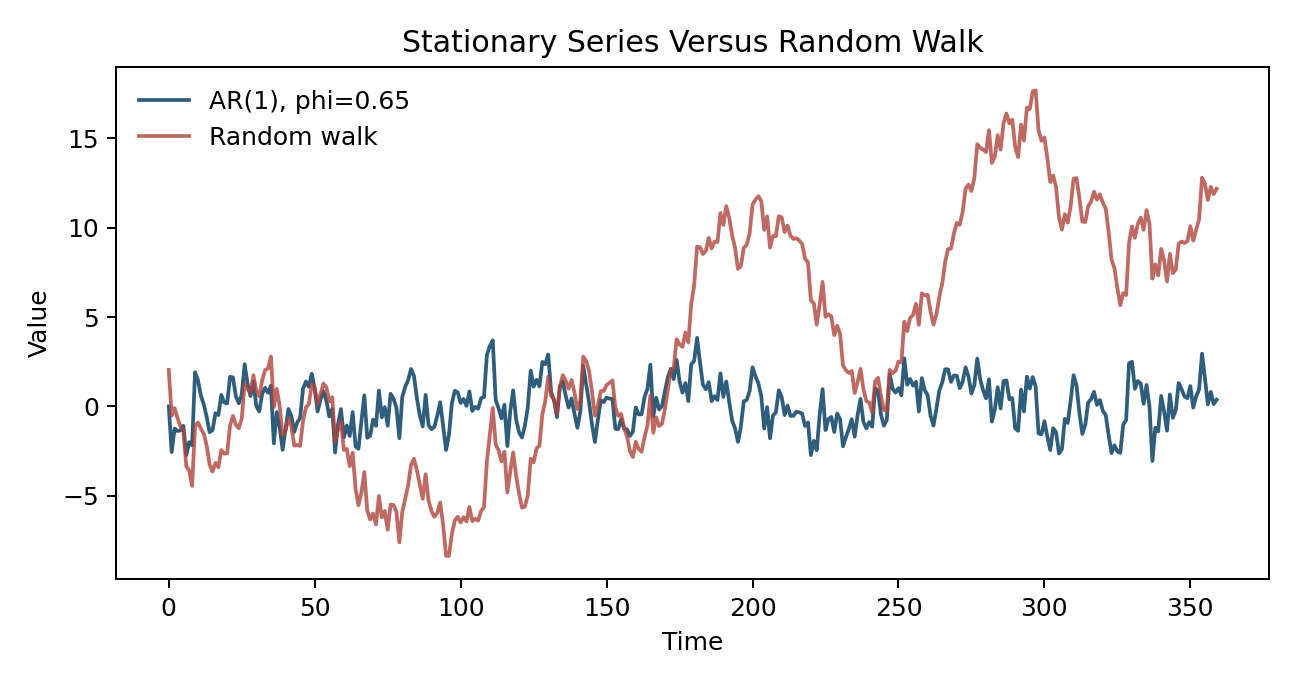
\includegraphics[width=0.86\textwidth]{ch03_fig01_stationary_vs_random_walk.png}
  \caption{平稳 AR(1) 与随机游走对比：平稳序列围绕固定均值波动，随机游走的水平随时间漂移。}
\end{figure}

\begin{figure}[htbp]
  \centering
  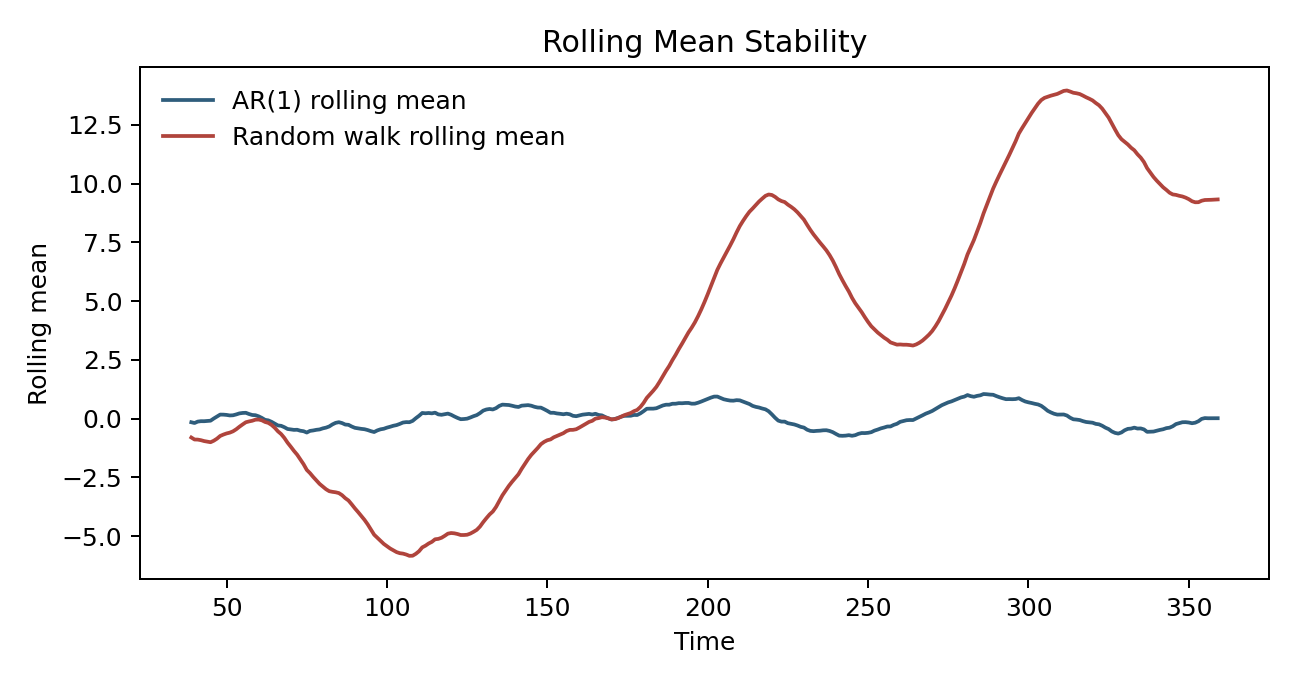
\includegraphics[width=0.86\textwidth]{ch03_fig02_rolling_mean.png}
  \caption{滚动均值稳定性：平稳序列的滚动均值较稳定，随机游走的滚动均值呈持续漂移。}
\end{figure}

\section{练习提要}

原文练习主要围绕下列方向展开：
\begin{itemize}
  \item 计算由白噪声构造的线性组合的协方差，练习协方差展开；
  \item 判断给定过程是否二阶平稳，并解释均值和协方差是否随时间改变；
  \item 为 SOI、太阳黑子和温度数据绘制 ACF，理解样本自相关的含义；
  \item 判断给定序列或函数是否可作为协方差。
\end{itemize}

\section*{本章小结}

第 3 章建立了全书的概率基础：时间序列推断依赖平稳性、遍历性和协方差结构。样本均值的标准误不再只由 \(c(0)\) 决定，而由所有滞后协方差共同决定；合法协方差必须满足非负定性，并可通过谱密度刻画。

\end{document}
